% ****** Start of file templateForReport.tex ******

% TeX'ing this file requires that you have all prerequisites
% for REVTeX 4.1 installed
%
% See the REVTeX 4 README file
% It also requires running BibTeX. The commands are as follows:
%
%  1)  latex templateForReport.tex
%  2)  bibtex templateForReport
%  3)  latex templateForReport.tex
%  4)  latex templateForReport.tex
%
\documentclass[%
 reprint,
%superscriptaddress,
%groupedaddress,
%unsortedaddress,
%runinaddress,
%frontmatterverbose,
%preprint,
%showpacs,preprintnumbers,
%nofootinbib,
%nobibnotes,
%bibnotes,
 amsmath,amssymb,
 aps,
%pra,
%prb,
%rmp,
%prstab,
%prstper,
%floatfix,
]{revtex4-1}
\usepackage{boxhandler}
\usepackage{graphicx}% Include figure files
\usepackage{dcolumn}% Align table columns on decimal point
\usepackage{bm}% bold math
\usepackage{hyperref}% add hypertext capabilities
\usepackage{natbib}
\usepackage{xcolor}
\usepackage{amsmath}
\usepackage{float}
\usepackage{siunitx}
\usepackage[labelfont=bf]{caption}
\usepackage{subcaption}
\bibliographystyle{abbrvnat}
\graphicspath{{figs/}}  
\newcommand{\btheta}{\boldsymbol{\theta}}
\usepackage[section]{placeins}

%\usepackage[mathlines]{lineno}% Enable numbering of text and display math
%\linenumbers\relax % Commence numbering lines

%\usepackage[showframe,%Uncomment any one of the following lines to test
%%scale=0.7, marginratio={1:1, 2:3}, ignoreall,% default settings
%%text={7in,10in},centering,
%%margin=1.5in,
%%total={6.5in,8.75in}, top=1.2in, left=0.9in, includefoot,
%%height=10in,a5paper,hmargin={3cm,0.8in},
%]{geometry}

\begin{document}

\title{Bayesian model selection}% Force line breaks with \\
%\thanks{A footnote to the article title}%

\author{Jakob Krause}
 \homepage{http://www.github.com/krausejm}
 \email{krause@hiskp.uni-bonn.de}
\author{Dominic Schüchter}
 \homepage{http://www.github.com/dschuechter}
 \email{dschuechter@uni-bonn.de}

\date{\today}% It is always \today, today,
             %  but any date may be explicitly specified

\begin{abstract}
\noindent This paper is an introduction to the concepts of \textsc{Bayesian} model selection. \textsc{Bayesian} statistics provide quantitative measures for model comparison, namely \textsc{Bayes} factor and \textsc{Bayes} complexity. The underlying theory and applications of those measures are shown as well as numerical techniques used in the process thereof.
\end{abstract}
\maketitle

%\tableofcontents

\section{\label{sec:intro}Introduction}
\noindent In physics, one is often faced with the problem of \emph{Model Selection} for a given data set. That means finding a mathematical description of the data, which on the one hand sufficiently characterizes the data structure and on the other hand satisfies the expected dependencies. This is by no means a trivial task; one has to understand the underlying physical model beforehand to not make the mistake of choosing a too complicated model although it may seemingly fit the data. At the same time too trivial assumptions can also lead in the wrong direction. Compactly this problem can be formulated in the following way (adapted from \cite[Chap. 4]{sivia}):

\begin{center}
	\emph{Alice has a theory; Bob also has a theory, but with an adjustable parameter $\lambda$. Whose theory should we prefer on the basis of data D?}
\end{center}



For this model-selection problem \textsc{Bayesian} inference provides quantitative measures, e.g. the \textsc{Bayes}-factor and the \textsc{Bayes}-complexity, these have among others been successfully used in astronomy as can be found in \cite{trotta,kunz,Trotta_2008} respectively. In this paper we will investigate two simulated example problems and apply various measures of bayesian model selection as to find out the true underlying model which was used to generate the simulated data. We will  focus on the numerical evaluation of such problems, especially\textsc{ Monte-Carlo} techniques.
\section{Theory}
\noindent In the following we will give a short introduction into \textsc{Bayes} theorem and the underlying concepts of parameter estimation and model selection.
\subsection{Bayes' Theorem}
\noindent The fundamental equation of \textsc{Bayesian} statistics -- for a dataset $y$ and parameters $\boldsymbol{\theta}$ -- is given by \textsc{Bayes} Theorem.
\begin{equation}
\label{eq:bayes}
\text{prob}(\boldsymbol{\theta} | y) =	p(\boldsymbol{\theta} | y) = \frac{p(y|\boldsymbol{\theta})\cdot p(\boldsymbol{\theta})}{p(y)} 
\end{equation}
Where $p(\boldsymbol{\theta} | y) $ is the posterior probability for parameters $\boldsymbol{\theta}$ given the data $y$, $p(y|\boldsymbol{\theta})$ is the likelihood that the data fits a model with parameters $\boldsymbol{\theta}$, $p(\boldsymbol{\theta})$ is the prior probability of $\boldsymbol{\theta}$ and $p(y)= \int_{-\infty}^{+\infty}\text{d}\boldsymbol{\theta} p(y|\boldsymbol{\theta})p(\boldsymbol{\theta})$ is the marginal likelihood which acts as a normalization.  In the case of parameter selection, the normalization can often be neglected since it is only a  constant. In the case of the model comparison it is a crucial quantity, as we will disuss in subsection (\ref{sec:Model_comparison}) \cite[Chap. 2]{sivia}. 

\subsection{Parameter estimation}
\noindent Assume we want to find the best parameters for a given dataset $y$ and model $M$. Eq. \eqref{eq:bayes} then can be written as
\begin{equation}\label{eq:PDF}
	p(\boldsymbol{\theta} | y,M) = \frac{p(y|\boldsymbol{\theta},M)\cdot p(\boldsymbol{\theta}|M)}{p(y|M)}.
\end{equation}
Evaluating this equation will give probability density functions (PDFs) 
\begin{equation}
\label{eq:marp}
	p(\theta_i|y,M)=\int p(\boldsymbol{\theta}|y,M)\prod_{j\neq i}\text{d}{\theta_j}
\end{equation}
 for each parameter $\theta_i$.  Because of equation \eqref{eq:marp} $p(\theta|D,M)$ is also called \emph{marginal posterior}. From this one can find the best fit value either by finding the value of $\theta$ for which the marginal posterior is maximized or by calculating the mean with respect to the marginal posterior.

\begin{align}
	\begin{split}
		p(\theta|y,M)=\max \Leftrightarrow \theta=\hat{\theta}\\
		\langle\theta\rangle=\int_{-\infty}^{\infty}\text{d}\theta  p(\theta|y,M)\cdot\theta
	\end{split}
\end{align}
Throughout this paper we will use $\langle\theta\rangle$ as our best fit estimate. \cite{sivia}

\subsection{Model comparison}\label{sec:Model_comparison}
\noindent To compare two (or more) competing models $M_i$ that describe a dataset $D$ let us write \textsc{Bayes} theorem once again
\begin{equation}
	p(M_i|y)=\frac{p(M_i)\cdot p(y|M_i)}{p(y)}.
\end{equation}
We recognize $p(y|M_i)$ as the marginal likelihood of the model $M_i$. Let now  the two competing models be those of Alice and Bob introduced in section \eqref{sec:intro}.Thus, $$p(y|M_i)=\int_{-\infty}^{\infty}\text{d}\lambda p(y|\lambda, M)\cdot p(\lambda|M)$$
follows \cite[Chap. 3]{sivia}.
\subsubsection{\textbf{Bayes Factor}}
One way of comparing two models is to compare their posterior odds, that is the ratio \cite{Trotta_2008} \begin{equation}\label{eq:bf}O_{ij}:=\underbrace{\frac{p(M_i|y)}{p(M_j|y)}}_{\text{posterior odds}}=\underbrace{\frac{p(y|M_i)}{p(y|M_j)}}_{\text{\textsc{Bayes} Factor}}\cdot\underbrace{\frac{p(M_i)}{p(M_j)}}_{\text{prior odds}}=B_{ij}\cdot\frac{p(M_i)}{p(M_j)}.\end{equation}
Usually we can assume the prior odds to be $\sim 1$ because we do not favor one model over the other just on prior beliefs. With this equation \eqref{eq:bf} simply becomes $$O_{ij}=B_{ij}.$$
Calculating $B_{ij}$ will be referred to as calculating the \textsc{Bayes} factor \emph{in favor of} model $M_i$. We can then evaluate the result of $B_{ij}$ as follows 
\begin{equation*}
	B_{ij}=B_{ji}^{-1}=\begin{cases} \geq 1 & \text{model } M_i \text{ favored}\\
	 <1 & \text{model } M_j \text{ favored}
	\end{cases}
\end{equation*}

Nevertheless a \textsc{Bayes} Factor $\geq1$ does not mean that the favored model is far superior. There is an empirical scale which points to the strength of evidence for a given $B_{ij}$. This is displayed in table \eqref{tab:bf}.


\begin{table}[htbp]

	\centering
	{\renewcommand{\arraystretch}{1.3}
	\begin{tabular}{|c|c|c|c|}
		\hline
		$|\ln B_{ij}|$& Odds & Probability & Strength of evidence \\
		\hline
		$< 1.0$& $ \lesssim 3:1$ & $< 0.750$  & Inconclusive  \\
		$1.0$ & $\sim 3:1$ & $0.750$ & Weak evidence  \\
		$2.5$& $\sim 12:1$ & $0.923$ & Moderate evidence \\
		$5.0$& $\sim 150:1$ & $0.993$ & Strong evidence \\
		\hline
	\end{tabular}}
\caption{Empirical scale for evaluating the strength of evidence when comparing two models $M_i$ vs. $M_j$, adapted from \cite{Trotta_2008}}
\label{tab:bf}
\end{table}
%{\color{red} Bayes factor vor allem attraktiv für genestete modelle}


\subsubsection{\textbf{Bayes Complexity}}
When comparing models with a different amount of parameters, we obviously denote more parameters as more complex. A fundamental question of model-selection is then if the given data supports more or less parameters. A na\"ive measure of complexity would be the number of free parameters a model has, we denote this as $\mathcal{C}_0$. A more sophisticated measure of complexity is given by the so called \textsc{Bayesian} complexity, first introduced by Spiegelhalter et al \cite{Spiegelhalter}, which can be written as \cite{kunz} 
\begin{equation}\label{eq:Bayes_Complexity}
	\mathcal{C}_b=-2\int \text{d}\boldsymbol{\theta} p(\boldsymbol{\theta}|y,M)\log(\mathcal{L}(\boldsymbol{\theta}))+2\log(\mathcal{L}(\boldsymbol{\tilde{\theta}})),
\end{equation}
with  the likelihood $\mathcal{L}(\boldsymbol{\theta})=p(D|\boldsymbol{\theta},M)$ and $\boldsymbol{\tilde{\theta}}=\langle\boldsymbol{\theta}\rangle$. $\mathcal{C}_b$ describes how many model parameters the data is able to constrain \cite{kunz} and is thus a useful tool for examining models with an increasing number of parameters. If we define a $\chi^2$ as $\mathcal{L}(\boldsymbol{\theta})\propto \exp(-\chi^2/2)$, we can write 
\begin{equation}\label{eq:Bayes_Complexity_alt}
	\mathcal{C}_b=\overline{\chi^2(\boldsymbol{\theta})}-\chi^2(\boldsymbol{\tilde{\theta}}),
\end{equation}
where $\overline{\chi}$ denotes the mean taken over the posterior PDF. 
The definition of $\mathcal{C}_b$ is chosen such that $\mathcal{C}_b\to\mathcal{C}_0$ for highly informative data \cite{kunz}.

\section{Methods}\label{sec:meth}
\noindent We will now describe the functions of the used algorithms for the model selection. Since the implementation of the so called nested sampling is sufficiently dealt with by another group \cite{paramter_fit} our implementation uses the \texttt{PyMC3}-Python Library \cite{PyMC3}.  \texttt{PyMC3} offers simple solutions to create models and a wide variety of sampling algorithms. Furthermore the \texttt{ArviZ}-Library provides methods for posterior analysis and visualization \cite{ArviZ}. Our code can be found \hyperref{https://github.com/dschuechter/physics760_schuechter_krause}{Github-Repository}{Bayes model selection}{here}.

 \subsection{Monte-Carlo Sampling}
\noindent First, the goal of \textsc{Monte-Carlo} sampling is discussed. Often equations \eqref{eq:marp}, \eqref{eq:Bayes_Complexity} and \eqref{eq:Bayes_Complexity_alt} have no closed analytical solutions, so we are left with a numerical ansatz (or analytical approximations) \cite{Toussaint}. One possibility is given by Markov-Chain-Monte-Carlo Sampling (MCMC) \cite{Toussaint}. The main idea is to generate a chain of parameter samples $\boldsymbol{\theta}^{(t)}$ that follow the posterior PDF \eqref{eq:PDF}. For such a chain the mean with respect to the posterior is given by 
 \begin{equation}
 	\langle \boldsymbol{\theta}\rangle\approx \int p(\boldsymbol{\theta} | y)\boldsymbol{\theta}d\boldsymbol{\theta}=\frac{1}{N}\sum_{t=0}^{N-1}\boldsymbol{\theta}^{(t)},
 \end{equation}
since the samples follow the PDF $p(\boldsymbol{\theta} | y)$. Analogously the expectation value of any function with respect to the posterior is
 \begin{equation}
	\langle f(\boldsymbol{\theta})\rangle\approx\frac{1}{N}\sum_{t=0}^{N-1}f(\boldsymbol{\theta}^{(t)}).
\end{equation}
Having established a \textsc{Markov} chain, one can compute the marginal posterior \eqref{eq:marp} by binning $\theta_i$ in the given parameter range and ignoring all other parameters \cite{Trotta_2008}. 

\subsection{Metropolis-Hastings Algorithm}
\noindent So far we have discussed what we gain from sampling from the posterior distribution. We have not yet explained an algorithm how this is actually achieved.  For our purposes we chose the \emph{Sequential Monte Carlo} sampling algorithm provided by \texttt{PyMC3} \cite{PyMC3_SMC}, because it grants easy access to the marginal likelihood. This in turn is needed for model comparison via the \textsc{Bayes}-factor. Because the \textsc{Metropolis-Hastings}-algorithm is one of the fundamentals of understanding SMC, see subsection \eqref{sec:SMC}, we briefly state it here. The main characterization of a \textsc{Markov} chain -- which consists of random parameters $\boldsymbol{\theta}^{(t)}$ -- is that each element is only determined by the previous element. In our case we want to sample in the parameter space according to the distribution $p(\btheta|y,M):=p(\btheta)$ \eqref{eq:PDF}. We can achieve this by randomly proposing a new vector in parameter space $\btheta'$  according to a arbitrary proposal distribution $p_p(\boldsymbol{a}|\boldsymbol{b})$ and accept it with a probability $$A(\btheta',\btheta^{(t)})=\min\left(1,\frac{p(\btheta')p_p(\btheta^{(t)}|\btheta')}{p(\btheta^{(t)})p_p(\btheta'|\btheta^{(t)})}\right).$$
This ensures the sampled values follow the desired PDF \cite{Toussaint}. This is only a very brief overview of MCMC. More information on the underlying theory can be found e.g. in \cite{neal}

\subsection{Sequential Monte Carlo (SMC)}\label{sec:SMC}
 \noindent Since the SMC algorithm joins several statistical concepts, including \emph{importance sampling}, \emph{tempering} and a MCMC kernel (\textsc{Metropolis-Hastings}) \cite{PyMC3_SMC}, it is a highly non-trivial algorithm. Thus, a detailed description is beyond the scope of this paper. We will now sketch the main idea of the algorithm. 
 First let us introduce an auxiliary \emph{temperature parameter} $\beta$ and write equation \eqref{eq:PDF} as 
   $$p(\btheta|y)_\beta=\frac{p(y|\btheta)^\beta\cdot p(\btheta)}{Z_\beta},$$
   with $Z_\beta=\int\text{d}\btheta p(y|\btheta)^\beta\cdot p(\btheta)$. For $\beta=1$ we get the same equation as before, that is $p(\btheta|y)_\beta=p(\btheta|y)$. The idea is to gradually sample from $\beta=0$ to $\beta=1$ using $\beta$ to control the transition from an easy to sample distribution to a harder one. The final result is a collection of samples from the true posterior \cite{PyMC3_SMC}. We can then estimate the marginal likelihood as \cite{SMC_PEPE} \begin{equation}\label{eq:with_the_hat}
   	\hat{p}(y)=\prod_{i}\widehat{\frac{Z_{\beta_i}}{Z_{\beta_{i-1}}}}.
   \end{equation}
     The hat denotes, that this is a numerical estimation of $p(y)$ \cite{SMC_PEPE}. Using SMC we can in one run do parameter inference and also compare different models using the \textsc{Bayes}-factor \eqref{eq:bf}.
 
\subsection{Savage Dickey Density Ratio (SDDR)} \label{subsec:sddr}
Now we introduce an alternative way of computing the \textsc{Bayes}-factor \eqref{eq:bf} for \emph{nested} models; Consider model $M_j$ with free parameters $\omega,\psi$ and a submodel $M_i$ with one free parameter $\psi$ and fixed $\omega=\omega_\star$. Let us further assume seperable priors (which is usually the case \cite{trotta}) $$p(\omega,\psi|M_j)=p(\omega|M_j)p(\psi|M_i).$$
We can then write the \textsc{Bayes}-factor as \cite{trotta} \begin{equation}
	\label{eq:sddr}
	B_{ij}=B_{ji}^{-1}=\frac{p(\omega|y,M_j)}{p(\omega|M_j)}\bigg|_{\omega=\omega_\star}  \text{\hfill (SDDR)}.
\end{equation}
\subsection{Error-analysis and diagnostics}
\noindent To evaluate the errors for the computed quantities we estimate the statistical error given by multiple \emph{Monte-Carlo} runs. Since the results matched our expectations, we are not considering systematic errors in our code. This can be said, because we chose the true models of the underlying data.

To check whether the \textsc{Markov} chains converge, we used the \texttt{ArviZ}-Library that provides functions to visualize \emph{marginal posteriors} and \textsc{Markov} chains \cite{ArviZ}. 
\section{Examples}\label{sec:examples}
\noindent We will now discuss two instructive examples applying the methods described in section \eqref{sec:meth}.

\subsection{Betabinomial example (coin flip)}\label{sec:coin}
\noindent Let us consider as a starting example, the flipping of a coin, i.e. an experiment where we can measure either heads ($H$) or tails ($T$) with $50\%$ probability, respectively. This, while simple, allows us an intuitive approach to Bayesian inference and model selection as well as to the MCMC techniques discussed before. Furthermore is this example easily altered to many problems with the option of either success or failure. Assume we throw a coin $N$ times.  Based on the outcome we wish to determine the probability for $H$ and draw a conclusion whether the coin is fair or, in fact, biased. We simulated data for $N=50$ and the biased coin with $p(H)=0.25$.
\subsubsection{\textbf{Analytical approach}}
\noindent Since this example is relatively simple we can compute the \textsc{Bayes}-factor also analytically.

Let us remember \textsc{Bayes} theorem in the context of this example where we want to compare two models $M_i,i=1,2$ which assign the following posterior to the probability of heads $p(\theta|y,M_i)$ for a given dataset $y$
$$p(\theta|y,M_i)=\frac{p(y|\theta,M_i)\cdot p(\theta|M_i)}{p(y|M_i)}.$$
Let now $M_1$ be a model which assumes a fair coin, so that the \emph{prior} is narrowly set around $\theta=0.5$. $M_2$ assumes a biased coin, that is a \emph{prior} centered around $\theta =0.25$. If we want to obtain the \textsc{Bayes}-factor we have to calculate $$p(y|M_i)=\int \text{d}\theta p(y|\theta,M_i)\cdot p(\theta|M_i) $$
because $B_{12}$ is given by \eqref{eq:bf} $$B_{12}=\frac{p(y|M_1)}{p(y|M_2)}.$$
To get an analytical solution we first have to assign \emph{prior} and \emph{likelihood} for each model. A natural ansatz for a prior $p(\theta|M_i)$ would be the \emph{Beta-distribution}, since it is limited to the finite interval $[0,1]$. Its PDF is given by \cite{kormaz} \begin{align*}f(\theta;\alpha,\beta)&=\frac{\Gamma(\alpha+\beta)}{\Gamma(\alpha)\Gamma(\beta)}\theta^{\alpha-1}(1-\theta)^{\beta-1}\\&:=\frac{1}{B(\alpha,\beta)}\theta^{\alpha-1}(1-\theta)^{\beta-1}.
\end{align*}
Where $\Gamma$ is the \emph{Gamma-function} \cite{gamma_function} and $B(\alpha,\beta)$ is the \emph{Beta-function} \cite{beta_function}.
To get a narrowly centered distribution around $0.5$ we chose $\alpha=\beta=50$. To get a distribution skewed around $0.25$ we have to choose $\beta=3\alpha-2$ \cite{wiki}, in our case $\alpha=5,\beta=13$, see figure \eqref{fig:beta_dist}.
\begin{figure}[htbp]
	\centering
	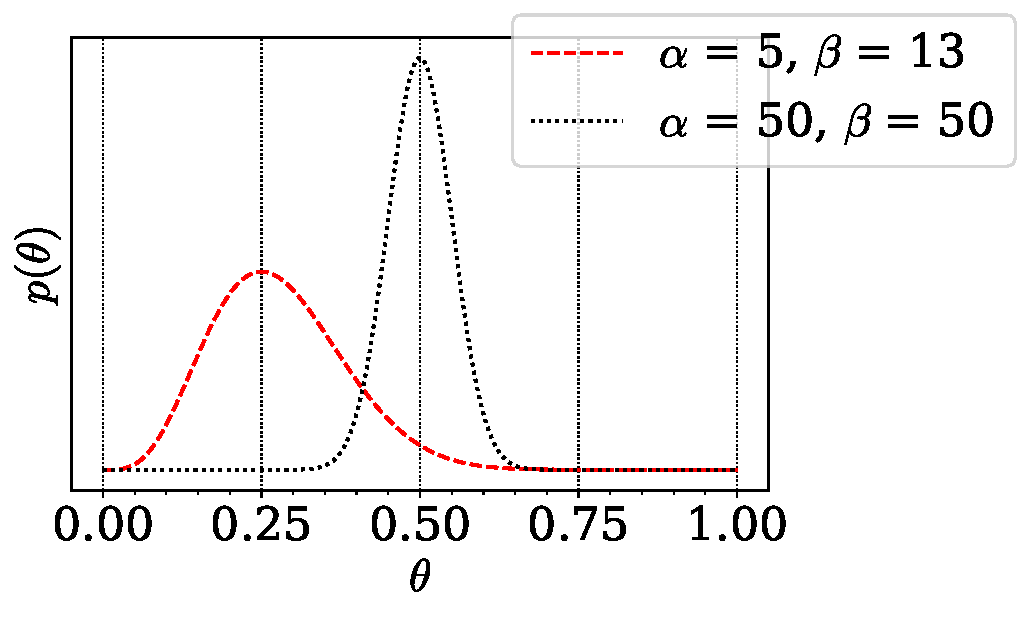
\includegraphics[width=\linewidth]{beta_dist}
	\caption{Beta-distribution as \emph{prior} $p(\theta|M_i)$ for the two different models}
	\label{fig:beta_dist}
\end{figure}
Now we will assign the \emph{likelihood} function $p(y|\theta,M)$. We can assume that each coin throw is independent of preceding coin throws and, naturally, only two outcomes are possible. Then a \emph{Binomial Distribution} is a suitable choice for our likelihood $p(y|\theta,M_i)$. If we observe $k$ heads out of $N$ coin throws ($y=(N,k)$) $$p(y|\theta,M_i)=\begin{pmatrix}N\\k
\end{pmatrix}\theta^k(1-\theta)^{N-k}.$$
Since we only are only interested in the ratio $B_{12}$ we can drop the binomial coefficient and write $$p(y|\theta, M_i)\propto \theta^k(1-\theta)^{N-k}.$$
Then the integral becomes \cite{PyMC3_BF}
\begin{align*}
	p(y|M_i)&\propto \int_{0}^{1} \text{d}\theta \frac{1}{B(\alpha,\beta)} \cdot \theta^{\alpha+k-1}\cdot (1-\theta)^{N-k+\beta-1}\\
	&=\frac{B(\alpha+k,\beta+N-k)}{B(\alpha, \beta)}.
\end{align*}
With this solution the \textsc{Bayes}-factor becomes
\begin{equation}\label{eq:anal_bf}
	B_{12}=\frac{B(\alpha_1+k,\beta_1+N-k)\cdot B(\alpha_2,\beta_2)}{B(\alpha_2+k,\beta_2+N-k)\cdot B(\alpha_1,\beta_1)}.
\end{equation}
For the biased coin $M_2$ should be superior. The analytical result of equation \eqref{eq:anal_bf} is $$B_{21}=B_{12}^{-1}=9.5839.$$

\subsubsection{\textbf{Numerical approach}}
\noindent We now compute the \textsc{Bayes}-factor numerically using the SMC-algorithm provided by \texttt{PyMC3}. We assigned the same \emph{priors} and \emph{likelikhoods} as in the analytical approach with a sample size of 2000 and 20 \textsc{Monte-Carlo} runs. The sampling yielded the \emph{marginal posteriors} depicted in figure \eqref{fig:coin_marp}. 
The \textsc{Bayes}-factor according to equation \eqref{eq:with_the_hat} evaluated to
$$B_{21}=B_{12}^{-1}=9.5829\pm0.4719$$
in very good agreement with the analytical result.
\begin{figure}[htbp]
	\begin{subfigure}{\linewidth}
		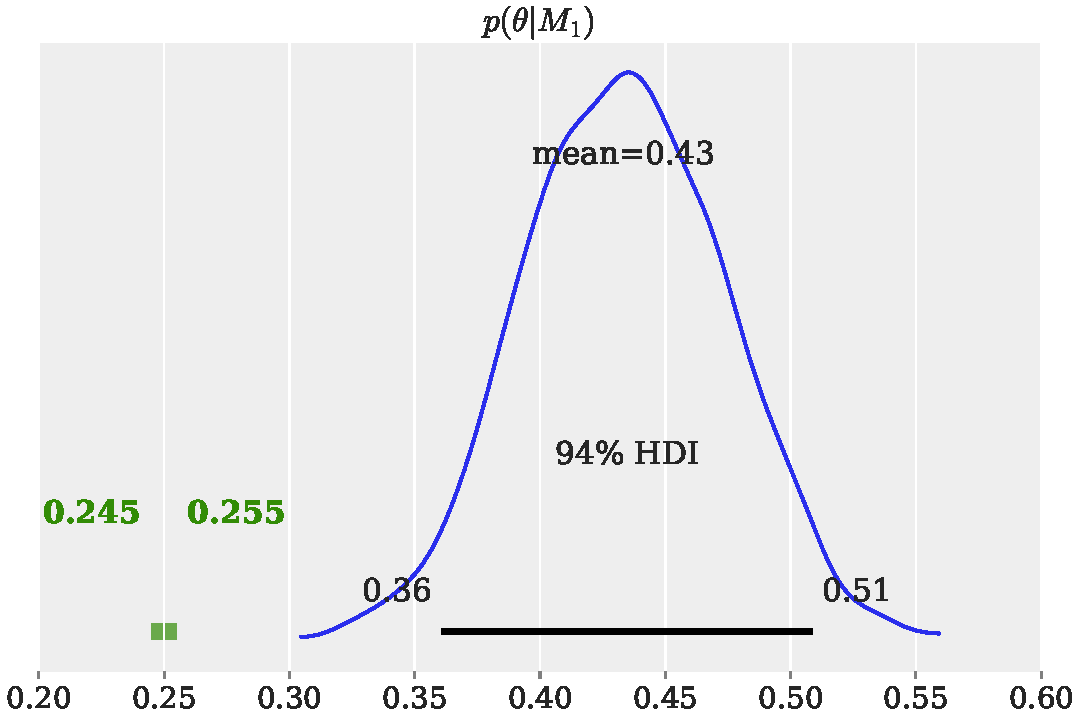
\includegraphics[width=0.9\linewidth]{coin_marp_m1.pdf}
		\subcaption{}\label{fig:coin_marp_a}
	\end{subfigure}
	\begin{subfigure}{\linewidth}
		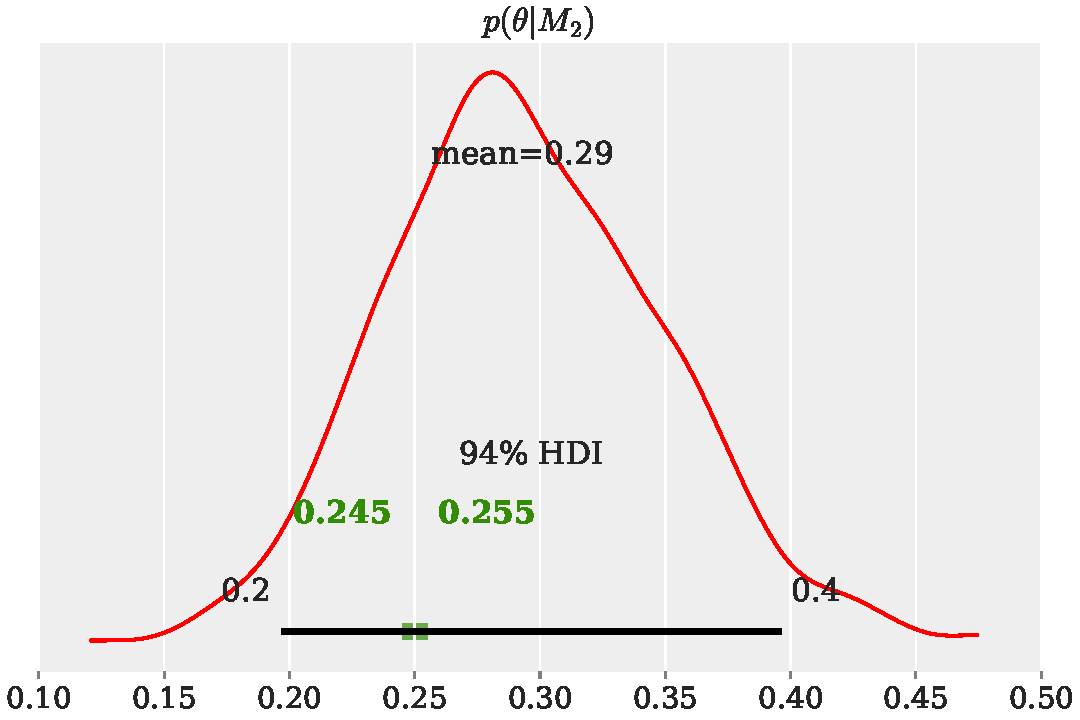
\includegraphics[width=0.9\linewidth]{coin_marp_m2.pdf}
		\subcaption{}\label{fig:coin_marp_b}
	\end{subfigure}
	\caption{The \emph{marginal posterior} for $\alpha=\beta=50$ \eqref{fig:coin_marp_a} and $\alpha=5, \beta=13$ \eqref{fig:coin_marp_b} of 2000 samples. HDI means highest density intervall. The highlighted green intervals denotes the expected value.}\label{fig:coin_marp}
\end{figure}
\subsection{Fitting a polynomial of unknown degree}\label{sec:poly}
\noindent A common problem in physics is to find an appropiate function to fit unknown data. In the following we will show how \textsc{Bayesian} model selection can help to answer this question. For that an example dataset -- following a polynomial of second order with a known variation of $\sigma=[0.7, 0.2]$ -- will be used and polynomials of first to third order will be considered as possible models. 
The true regression line is given by
\begin{equation*}
	f(x;\btheta)=a\cdot x^2+b\cdot x+c=2\cdot x^2+3\cdot x+1.
\end{equation*}
To tackle this problem numerically via the SMC algorithm, we have to assign \emph{priors} and \emph{likelihoods}. The \emph{priors} for the fit-parameters $a,b$ and $c$  are each described by a normal distribution with $\mu_{\text{prior}}=0$ and $\sigma_{\text{prior}}=2$, because we have some intuition what the parameters might be. That means $p(\btheta|M_i)=p(\theta_1|M_i)\cdot p(\theta_2|M_i)\cdots $. For the \emph{likelihood} functions we used normal distributions because we considered the noise being gaussian. The \emph{likelihood} can then be written as \cite[Chap. 3]{sivia}
$$p(y|\btheta, M_i)=\prod_{k=1}^{N}\frac{1}{\sigma\sqrt{2\pi}}\exp{\left[-\frac{(f(y_k;\btheta)-y_k)^2}{2\sigma^2}\right]}.$$
According to \textsc{Bayes} theorem we generated 2000 samples following the \emph{posterior} PDF $p(\btheta|y,M_i)\propto p(y|\btheta, M_i)\cdot p(\btheta|M_i) $ using the SMC algorithm. The resulting functions with parameters $a,b$ and $c$ in the highest density intervals (HDI) containing 99\% of the sampled values are displayed in figure \eqref{fig:HDI_sigma_07} for $\sigma=0.7$.
\begin{figure*}
	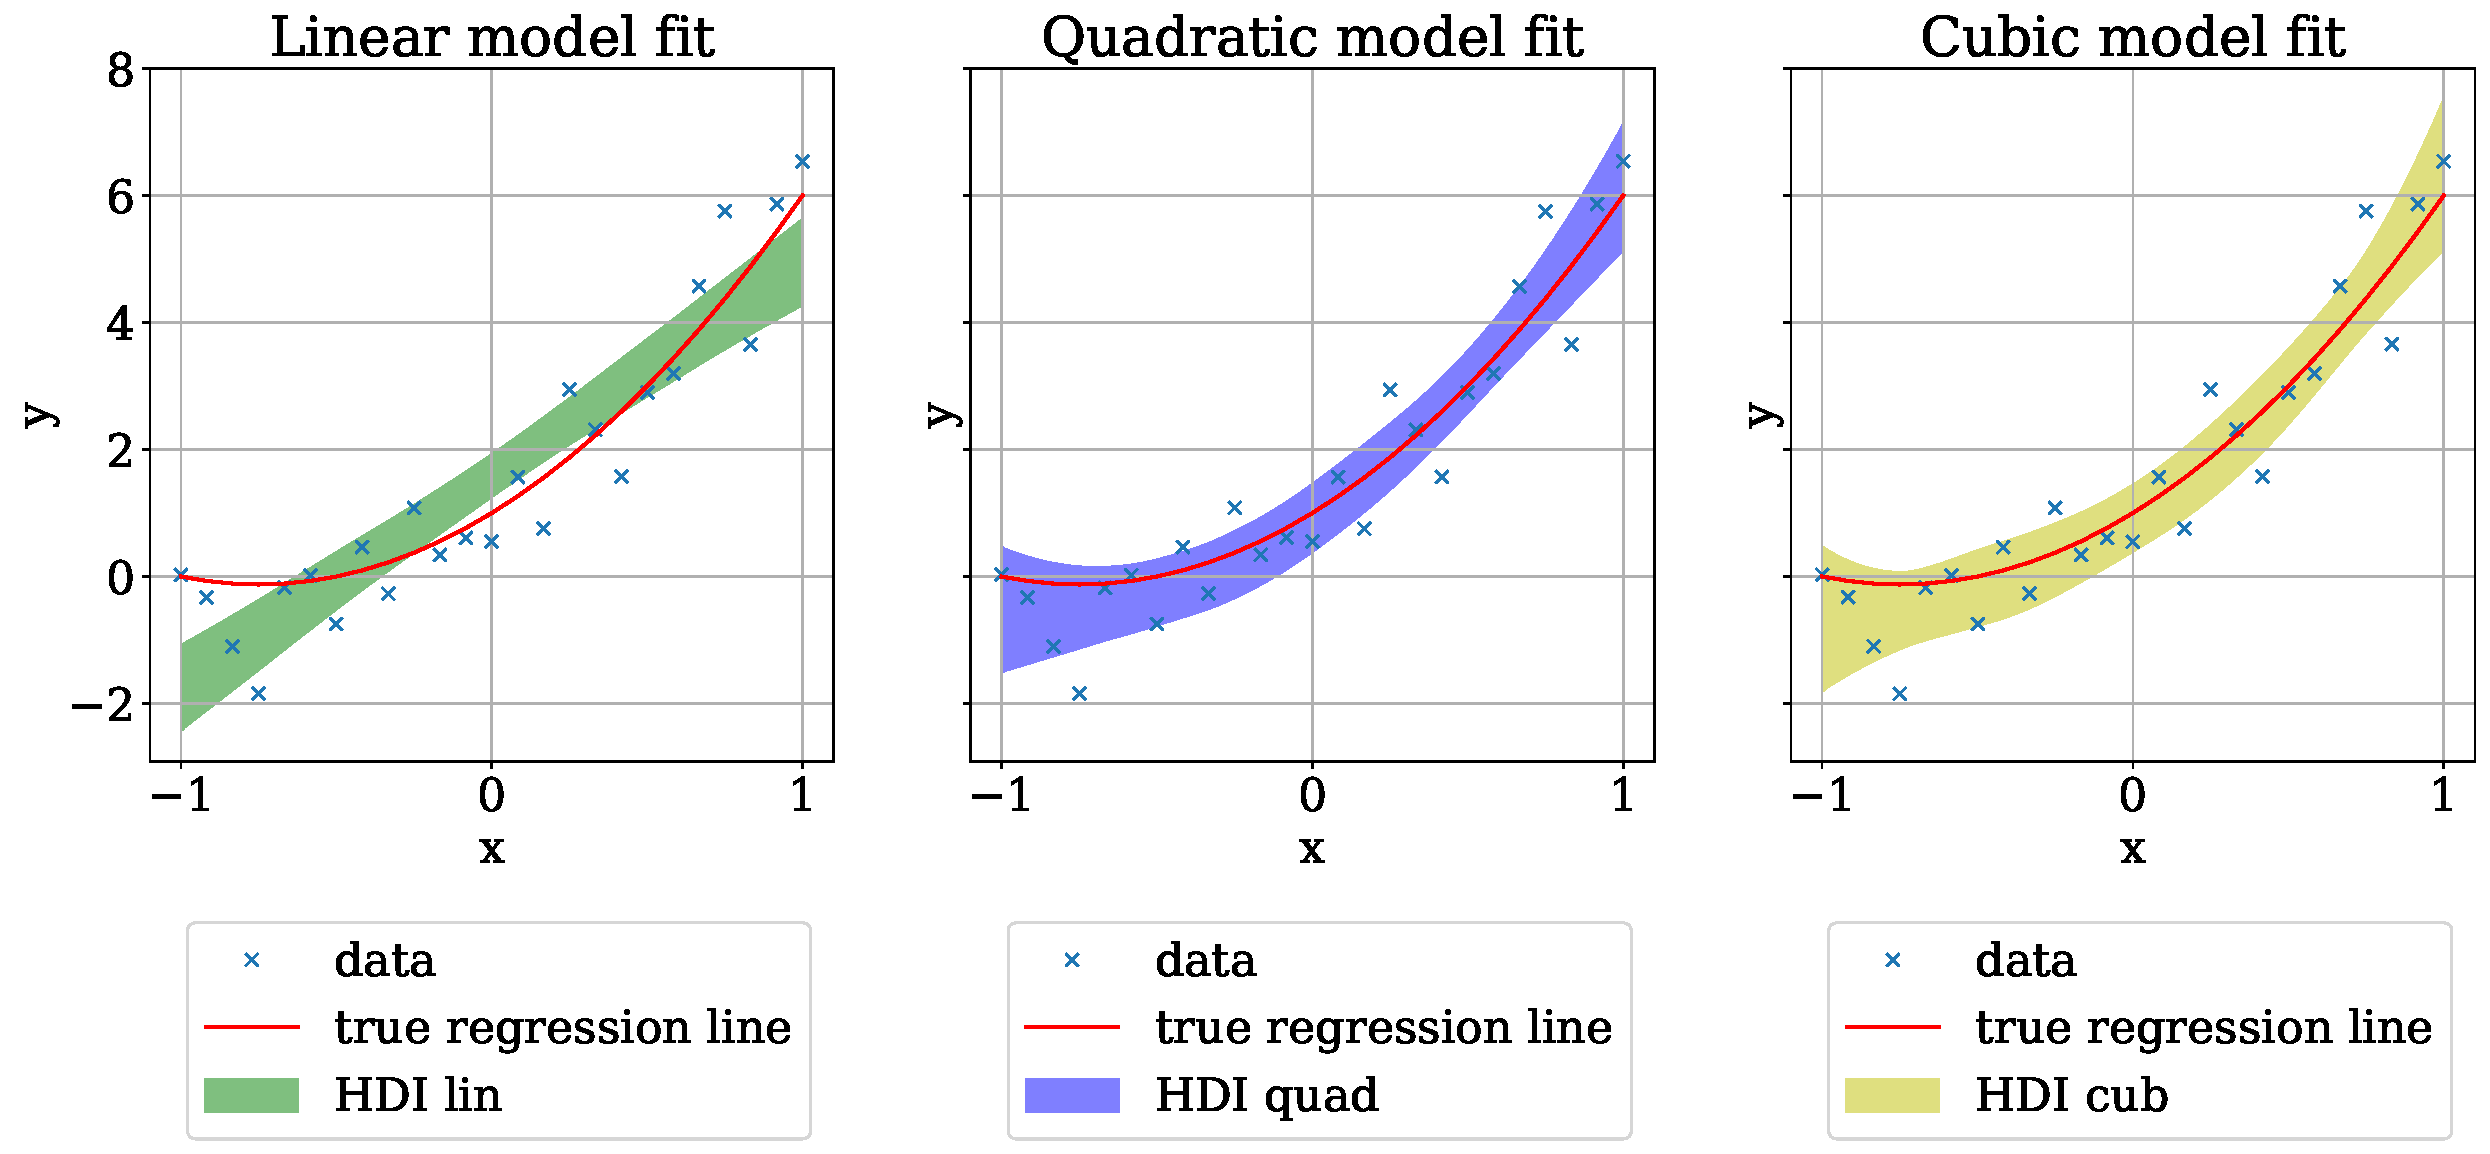
\includegraphics[width=\textwidth]{HDI_sigma_07}
	\caption{Result of parameter estimation with SMC. The data was generated with $\sigma=0.7$}\label{fig:HDI_sigma_07}
\end{figure*}
\subsubsection{\textbf{Bayes-factor via SMC}}
\noindent As before, it is now straightforward to compute the \textsc{Bayes}-factor comparing the models. Our results are listed in table \eqref{tab:res_smc}.

\begin{table}[H]
	{\renewcommand{\arraystretch}{1.3}
		\begin{tabular}{|c|c|c|}
			\hline
			Comparison $M_1$ vs. $M_2$ & $\ln(B_{12}(\sigma=0.7))$& $\ln(B_{12}(\sigma=0.2))$  \\
			\hline
			square vs. linear& $8.5507\pm0.053$&$119.1875\pm0.1394$\\
			cubic vs. linear & $7.6225\pm0.094$&$117.0686\pm0.1481$\\
			square vs. cubic&$0.9371\pm0.1093$ &$2.1249\pm0.10413$\\
			\hline
	\end{tabular}}
	\caption{Results of \textsc{Bayes}-factor via SMC}
	\label{tab:res_smc}
\end{table}

\begin{figure}[H]
	\centering
	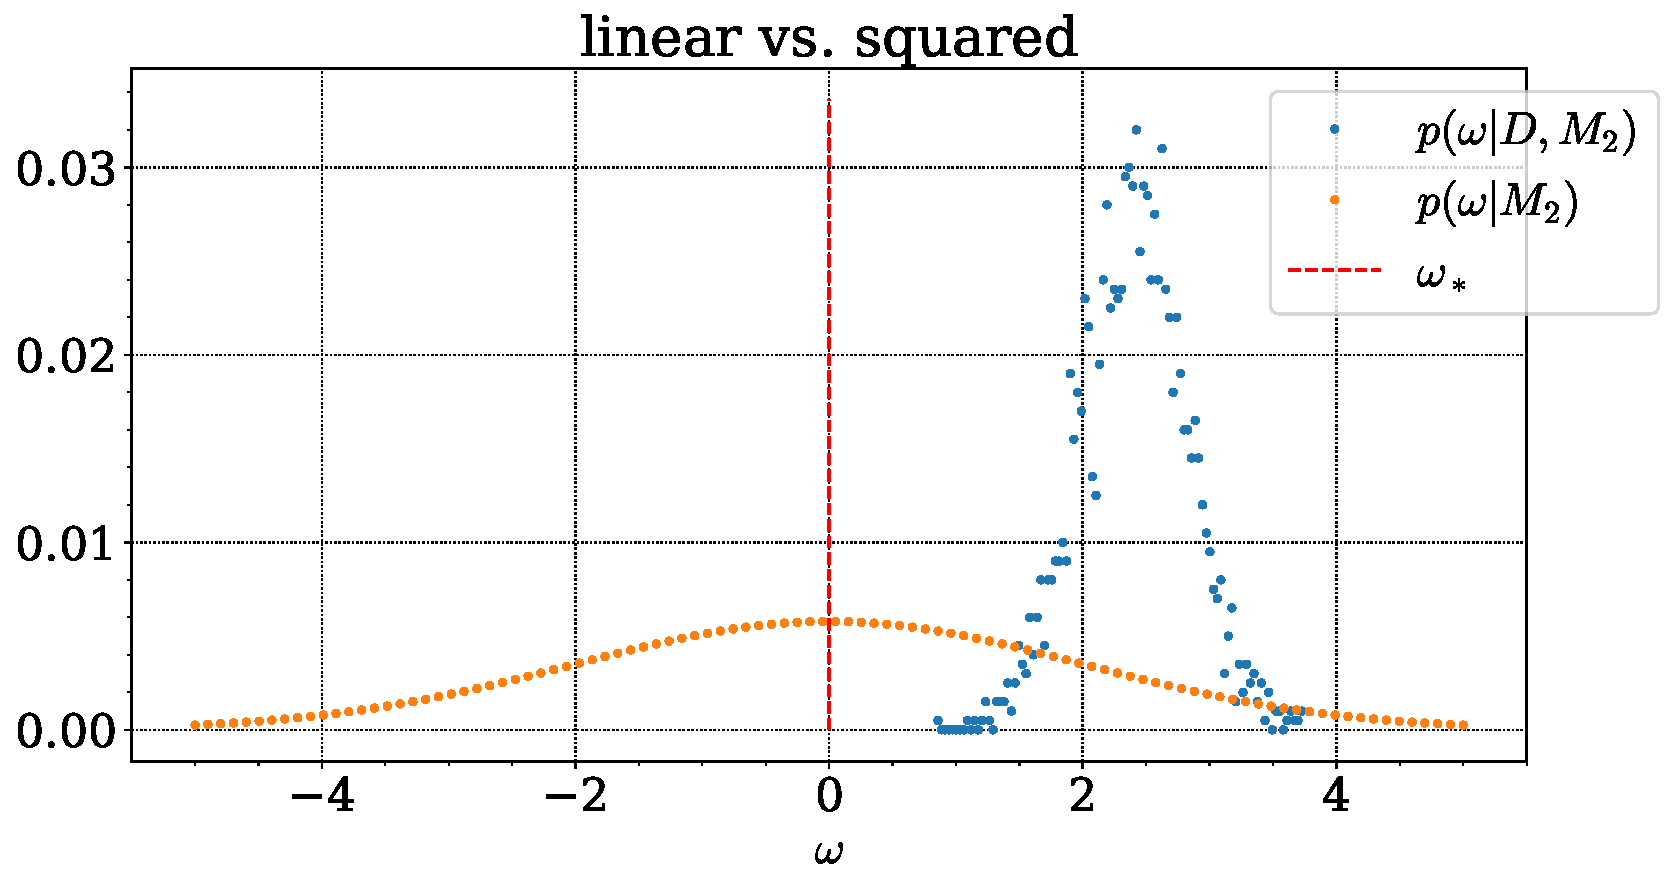
\includegraphics[width=0.9\linewidth]{SDDR_linear vs. squared_sigma_07a+.pdf}
	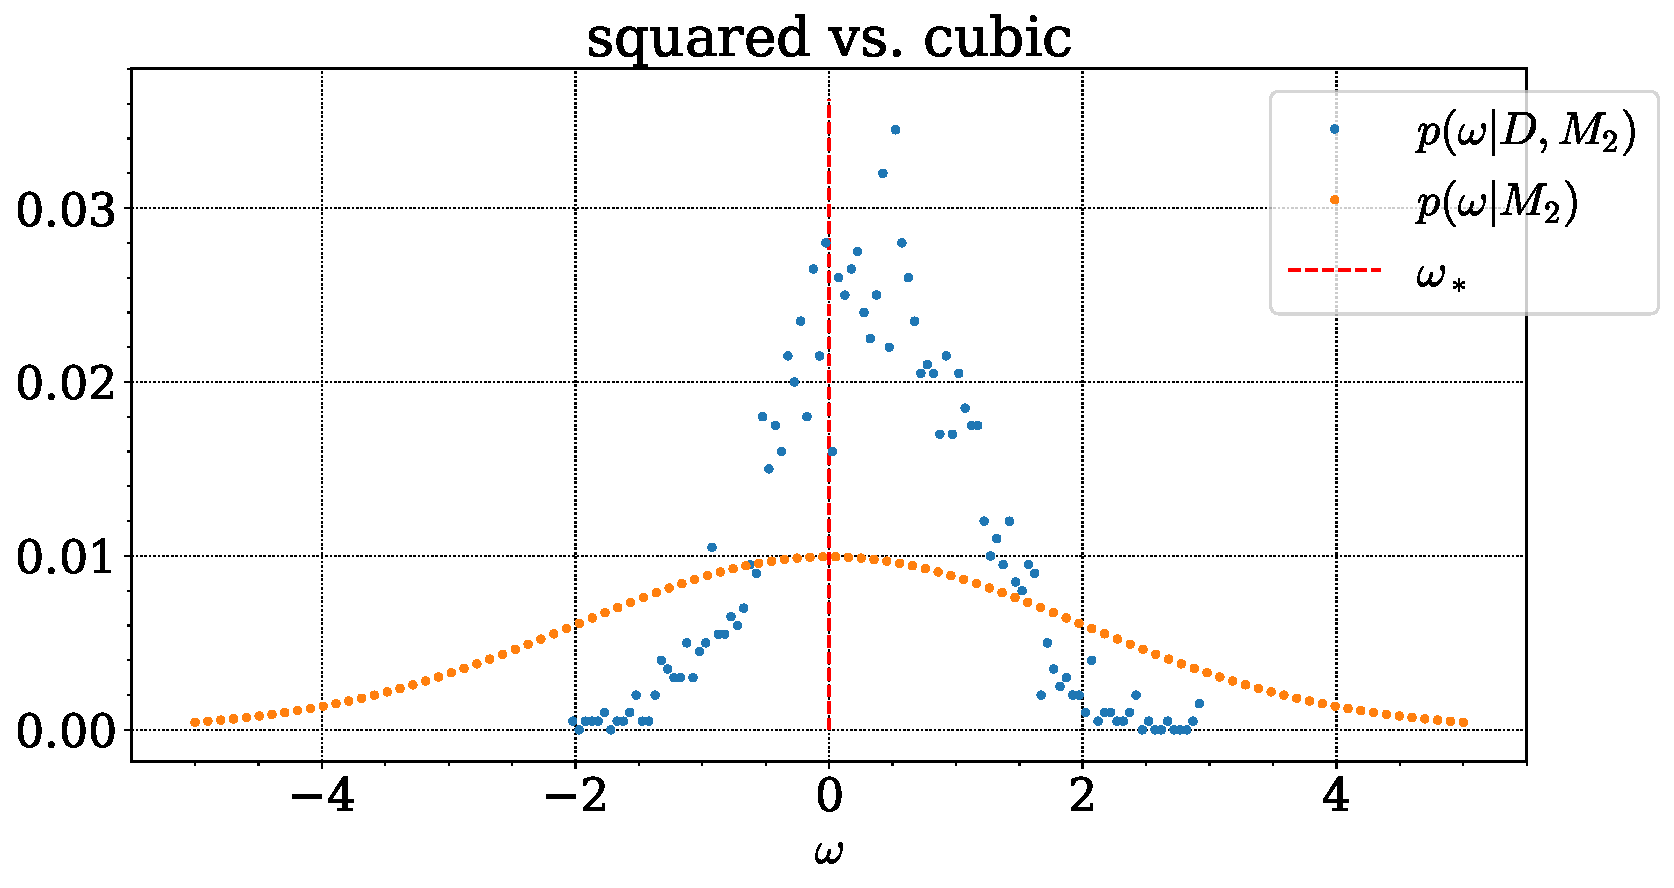
\includegraphics[width=0.9\linewidth]{SDDR_squared vs. cubic_sigma_07a+.pdf}
	\caption{Computation of the SDDR  ($\sigma=0.7$)}
	\label{fig:sddr}
\end{figure}

\begin{table}[H]
		{\renewcommand{\arraystretch}{1.3}
			\begin{tabular}{|c|c|c|}
				\hline
				Comparison $M_1$ vs. $M_2$ & $\ln(B_{12}(\sigma=0.7))$ & $\ln(B_{12}(\sigma=0.2))$ \\
				\hline
				square vs. linear& $>2.4301\pm0.27613$&$>2.0624\pm0.3077$\\
				square vs. cubic&$0.8091\pm0.0265$  &$2.1184\pm0.0723$\\
				cubic vs. linear & $>0.3329\pm0.1292$&$>1.0272\pm0.1572$\\
				\hline
	\end{tabular}}
	\caption{Results of \textsc{Bayes}-factor via SDDR. Note that for the comparison square vs. linear we could only provide a lower bound because our sample size did not provide us with values around $\omega_\star$. We compared the ratio of the \textsc{Bayes}-factors of square vs. linear and square vs. cubic to get the \textsc{Bayes}-factor of cubic vs. linear.}
	\label{tab:res_sddr}
\end{table}
\subsubsection{\textbf{Bayes-factor via SDDR}}
\noindent In section \eqref{subsec:sddr} we discussed an alternative way of computing the \textsc{Bayes}-factor. We notice this simplification applies to the case of polynomials of different degrees. Here each simpler model follows from the next more complex one by setting the coefficient of highest order to $0$. Also the criterion of seperable priors applies. It is now a simple task to evaluate equation \eqref{eq:sddr}. We only need the normalized \emph{marginal posterior} of the highest order coefficient and its corresponding prior at $0$. The prior is known and the marginal posterior is directly obtained once we have sampled and can then be normalized. In figure \eqref{fig:sddr} we show the priors and \emph{marginal posteriors} of the highest order coefficient of the polynomial of second and third order respectively, which leads us to the following results, see table \eqref{tab:res_sddr}.

\begin{figure}[H]
	\centering
	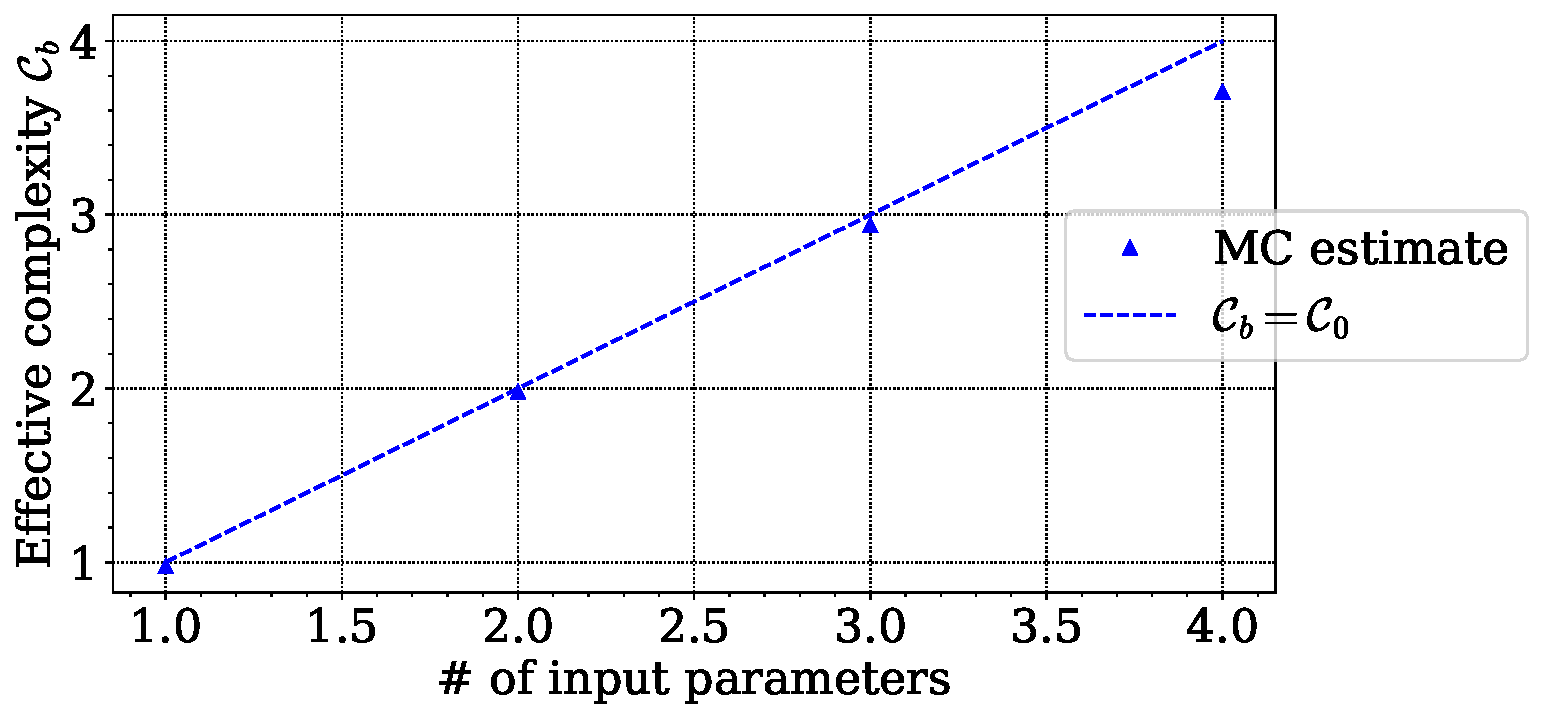
\includegraphics[width=\linewidth]{_sigma_07acomplexity.pdf}
	\caption{\textsc{Bayesian} complexity as a function of number of input parameters ($\sigma=0.7$)}
	\label{fig:complex}
\end{figure}

\vspace{-1.2cm}
\subsubsection{\textbf{Bayes-Complexity}}
\noindent As another measure of model selection, the \textsc{Bayesian} complexity $\mathcal{C}_b$ was introduced. Having sampled in parameter space $\btheta^{(t)}$, equation \eqref{eq:Bayes_Complexity_alt} is evaluated instantly as \cite{wuerz} \begin{align*}\mathcal{C}_b=&\frac{1}{N_S}\sum_{t=0}^{N_S-1}\left(\sum_{k=0}^{N_y-1}\frac{[y_k-f(y_k;\btheta^{(t)})]^2}{\sigma^2}\right)\\&-\sum_{k=0}^{N_y-1}\frac{[y_k-f(y_k;\frac{1}{N_S}\sum_{t=0}^{N_S-1}\btheta^{(t)})]^2}{\sigma^2}.\end{align*}
In figure \eqref{fig:complex} we plotted the computed complexity $\mathcal{C}_b$ as a function of the number of parameters and also the input complexity $\mathcal{C}_0$.


\section{Discussion}
\noindent We now discuss the results obtained in section \eqref{sec:examples}.
\subsection{Betabinomial example}
\noindent The analytical and numerical result are matching until the third decimal, while the analytical lies within the estimated statistical error. We were able to reproduce the expected results by using \textsc{Bayesian} inference.  By using table \eqref{tab:bf} we can say with weak to moderate confidence that the coin is biased. By using a bigger dataset, the confidence would rise. The marginal posteriors of figure \eqref{fig:coin_marp} indicate that the choice of \emph{priors} determines the best fit value. While model $M_1$ with the \emph{prior} centred around  $\theta=0.25$ achieves to include the true value (highlighted in green) in its 94\% HDI, model $M_2$ doesn't have enough data to discard its prior belief. 
\subsection{Fitting a polynomial of unknown degree}
\noindent To interpret the found results of the \textsc{Bayes} factor we consult table \eqref{tab:bf}. One can see that for both $\sigma$ the linear model is clearly disfavoured with strong evidence. For $\sigma=0.7$ we find inconclusive evidence if the square or cubic model is superior to the other. With $\sigma=0.2$ we find weak to moderate evidence that the square model is favoured. This is a result of the small variance of datapoints and the fact that a simpler model is generally favoured with the \textsc{Bayes} factor \cite{sivia}.This result is as we expected, since the underlying model is a polynomial of second order. 

The same can be said about the SDDR, although we could only find lower limits for the linear model in comparison to the others. This could be circumvented by choosing a bigger sample size or $\sigma$. The second proposal is not usable for real world data. We did not make use of a bigger sample size because we did not want to focus on the SDDR and only use it as a sanity check for the \textsc{Bayes} factor. Never the less we can say, that the results of the SDDR method are consistent with the results of the SMC method.

Since all errors are relatively small, we can conclude again that the \textsc{Markov} chains sufficiently converged.

Using figure \eqref{fig:complex} one can see, that the effective complexity $\mathcal{C}_b$ diverges for a number of parameters $\dim{\btheta}>3$. The data is not able to constrain more parameters than three. Using this information and the obtained \textsc{Bayes} factors one can confidentially assume, that the underlying model is a polynomial of second order. 

We chose a rather simple model that can easily be scaled up for higher order polynomials. The benefit of the shown simpler model is, that the reader can easily follow the chain of thought.  

\section{Summary}
\noindent In this paper we investigated the problem of \textsc{Bayesian} model selection. After introducing the needed theory of \textsc{Bayes} theorem, parameter estimation and model comparison we established two measures of \textsc{Bayesian} model comparison, namely \textsc{Bayes} factor and \textsc{Bayes} complexity. As a method to evaluate these the SMC algorithm and the \textsc{Savage Dicky} Density Ratio were introduced. First we studied the example of a biased coin flip. We could successfully use the \textsc{Bayes} factor to obtain a weak to moderate strength of evidence about the coin bias, see section \eqref{sec:coin}. As a second example we studied data distributed by a polynomial of second order with applied gaussian noise of two different magnitudes. We then used \textsc{Bayesian} inference to fit polynomials of order one to three. Again we could successfully derive that the polynomial of second order is the with moderate to strong evidence the correct model by using \textsc{Bayes} factor, \textsc{Savage Dicky} density ratio and \textsc{Bayes} complexity, see \eqref{sec:poly}. Having now established intuition for \textsc{Bayesian} model selection, one could apply those methods to experimental data and complex problems.


\noindent 
\FloatBarrier
\bibliography{refs}
\end{document}
%
% ****** End of file templateForReport.tex ******
